\documentclass[11pt]{article}
\usepackage{tikz}
\usepackage{xfrac}
%\usepackage{hyperref}
\usepackage[export]{adjustbox}
\def\checkmark{\tikz\fill[scale=0.4](0,.35) -- (.25,0) -- (1,.7) -- (.25,.15) -- cycle;} 
\usepackage{proj} 	% pull in style header
\usepackage{array}
\usepackage{sectsty}

\lhead{ECE540: SoC Design with FPGA's}

%TODO: Put in coverpage from hw1, with tunnel vision image.  

%----------------------------------------------------------------------------------------
%	TITLE SECTION
%----------------------------------------------------------------------------------------


\newcommand{\horrule}[1]{\rule{\linewidth}{#1}} % Create horizontal rule command with 1 argument of height

\title{	
\normalfont \normalsize 
\textsc{\LARGE Portland State University}\\[1.5cm] % Name of your university/college
\textsc{\Large SoC Design With FPGAs}\\[0.5cm] % Major heading such as course name
\textsc{\large ECE540}\\[0.5cm] % Minor heading such as course title
%\textsc{Portland State University} \\ [25pt] % Your university, school and/or department name(s)
\horrule{1.2pt} \\[0.4cm] % Thin top horizontal rule
\huge Tunnel Vision \\ % The assignment title
\horrule{1.2pt} \\[0.5cm] % Thick bottom horizontal rule
}

%----------------------------------------------------------------------------------------
%	AUTHOR SECTION
%----------------------------------------------------------------------------------------


\begin{document}\raggedright
\author{Erik Rhodes \and Bhavana Dhulipala \and Rohan Deshpande \and Nikhil Patil} % Your name
\maketitle % Print the title
\thispagestyle{empty}
\cfoot{\textit{Page \thepage { of} \pageref{LastPage}}}
\lhead{ECE540: SoC Design}
\chead{github.com/rhodeser/tunnel-vision}
\rhead{Tunnel Vision}


\begin{figure}[h]\centering

\includegraphics[height=0.65\textwidth]{Images/start.png}
	%\caption{Gameplay Block Diagram}
		\label{start}
	\end{figure}

\tableofcontents

%
%\title{\textbf{ECE540: Final Project}\\Tunnel Vision}
%\author{Erik Rhodes and Bhavana Dhulipala}
%\date{February 4, 2014}

%\begin{document}
%	\maketitle{}
%	\thispagestyle{empty}
%	\newpage 
%	
%%		\thispagestyle{empty} % back of cover page is blank
%%		\vspace*{0.5\paperheight}
%%		\begin{center}
%%		{\it This page intentionally left blank}
%%		\end{center}
%%		\newpage
%		\begin{center}
%			\tableofcontents
%			\newpage
%	\end{center}


%Start of Document

% PUT IN CODE?
% put in design specs - Pictures: Top module, Hardware specifications?

\section{Introduction} 
\textbf{Tunnel Vision} is a racing game that can be played on the \textbf{Xilinx Nexys3 FPGA} board and be displayed on a VGA monitor.

\subsection{Gameplay}
The player tries to avoid hitting the walls as it travels down the tunnel by moving the vehicle left and right. The space in between the walls steadily decreases until the player hits a wall or obstacle. The score is based on the amount of time the vehicle remains ``alive'', and is displayed on the 7-segment display.

\subsection{Controls}
The player can move his vehicle by using the left and right pushbuttons on the Nexys3. When the game is over, hitting the middle button will reset the course. The top button starts the game and the bottom pushbutton pauses it. Different icons and speeds can be selected by toggling the switches on the board.

		\begin{figure}[h]\centering
		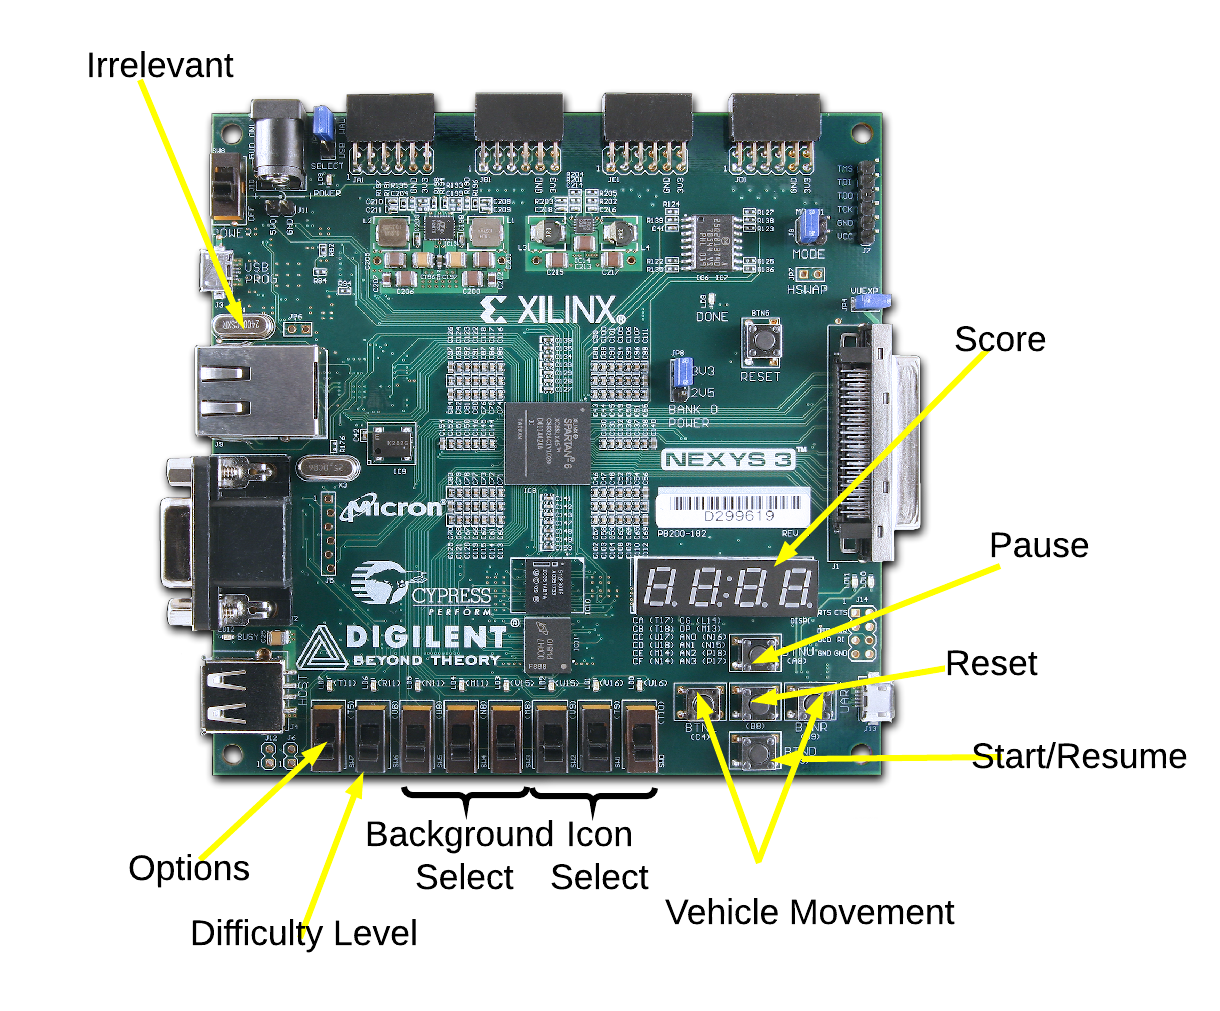
\includegraphics[height=0.8\textwidth, width=0.8\textheight]{Images/controls_mockup.png}
		\caption{Player Controls}
			\label{controls}
		\end{figure}	
	 	

\subsection{Features}
\textbf{Tunnel Vision} features both starting and ending screens. The courses are generated randomly through a pseudo-random number generator. Additionally, the LEDs are lit with certain patterns depending on the action the player is taking. If the player selects the harder difficulty, the score is incremented at a faster rate and with a multiplier, awarding them a higher score for the same distance traveled.
	

\section{Implementation}

	\begin{figure}[h]\centering
	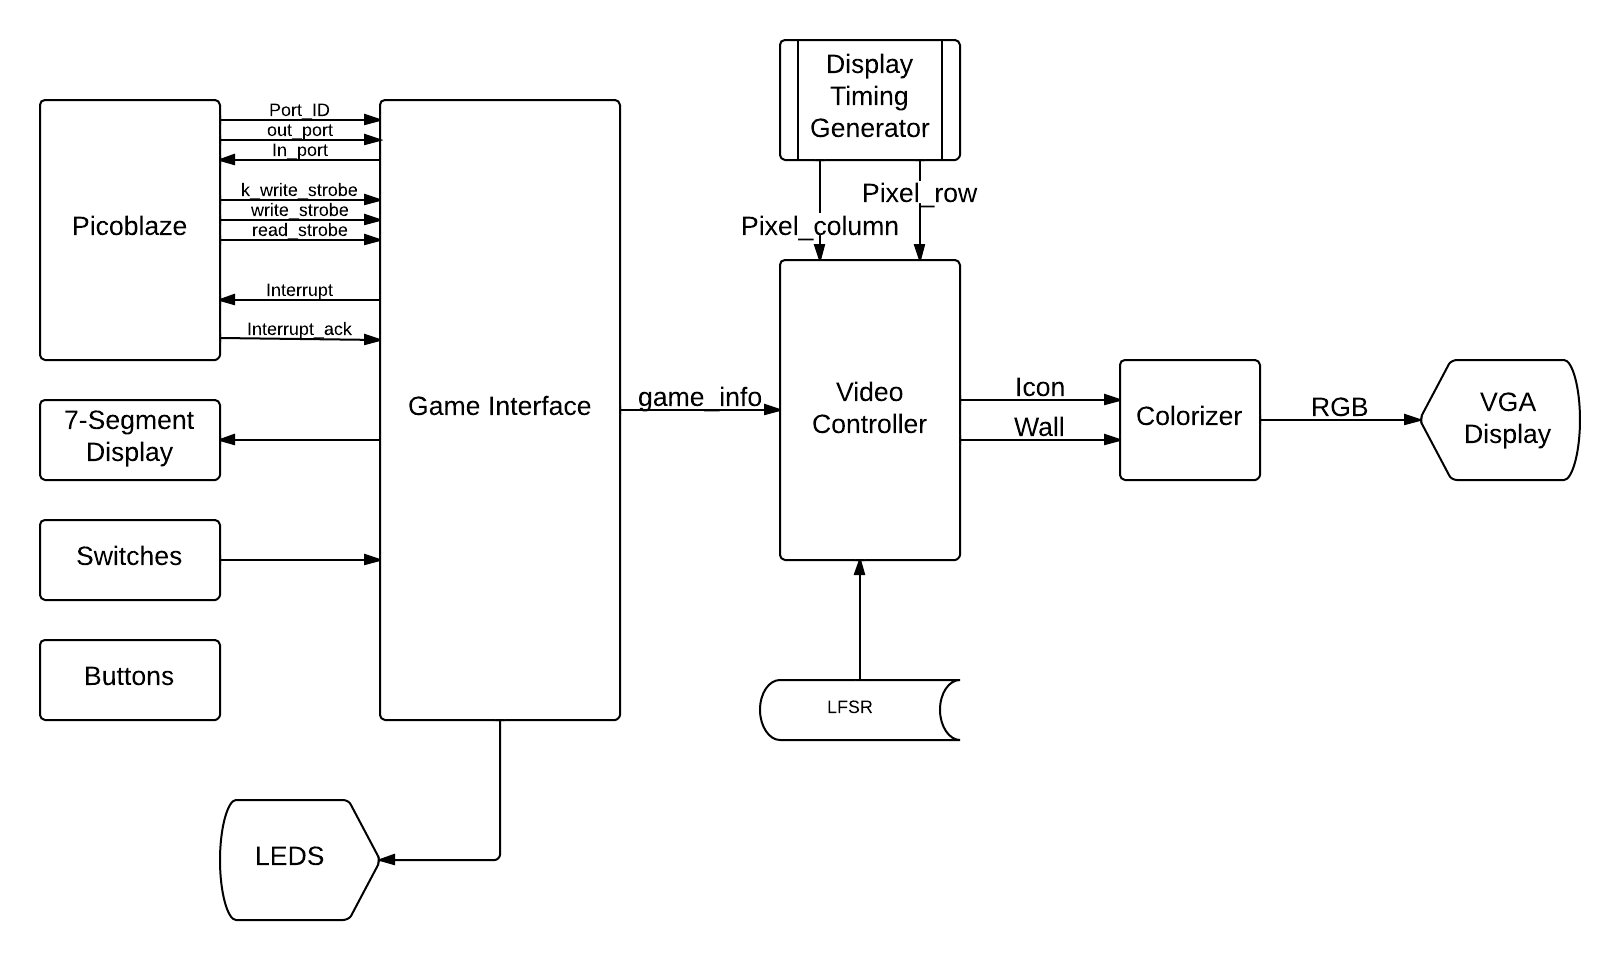
\includegraphics[height=0.7\textwidth, width=0.7\textheight]{Images/gameplay_diagram.png}
	\caption{Game play Block Diagram}
		\label{block_diagram}
	\end{figure}	

General overview of how things communicated, what was done in hardware vs soft core. 
		
The information controlled in the \textbf{PicoBlaze} core is sent to the \texttt{Video\_controller} module via the \texttt{game\_interface} module.  This information is constructed in an 8-bit register called \texttt{game\_info}.  The allocation of bits is seen in Figure \ref{game_info_bits}.

					
		\begin{figure}[h]\centering
		  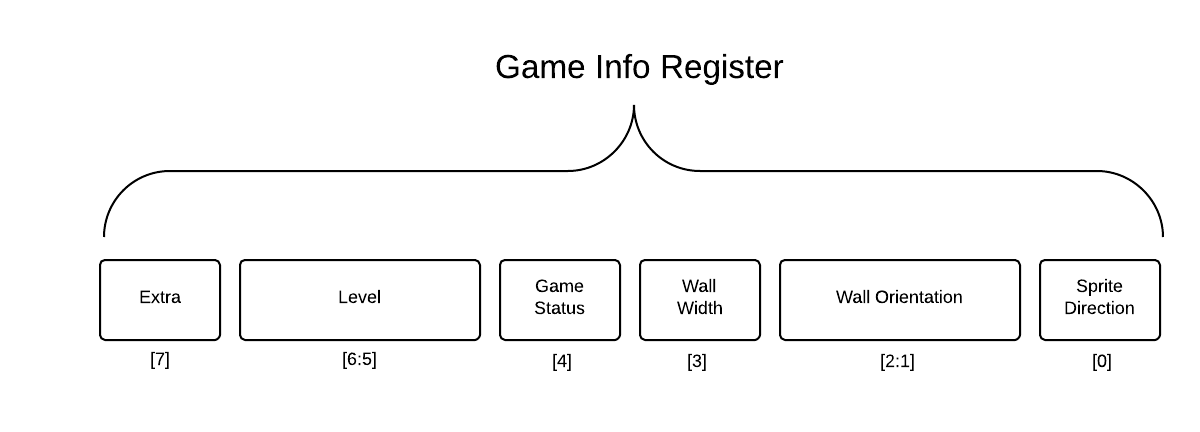
\includegraphics[width=.8\textwidth]{Images/game_info_bits.png}
		  \caption{Allocation of bits in game\_info register}
		  \label{game_info_bits}
		\end{figure}		
		
\subsection{Software}

Include Picoblaze diagram. \\ 
Collisions, obstacles, and icon changes were controlled in hardware.\\

In order to ensure the correct flow of game play, the push button inputs were checked in the other seen in Figure (......).  Each button check performs approximately the same function.  The pushbutton input is checked, all other bits not pertaining to the specific button are masked off, and the button value is checked.  If it has not been pressed, the next button check is called.  If it has been pressed, the state is updated accordingly and the LEDs output the desired pattern. 


\begin{lstlisting}[caption=Function checking if the top button has been pushed, label=chk_up_btn]		
		FETCH	  s2,		SP_BTN				;load saved debounced button
		AND		s2,		MSK_BTN_UP				;mask with up button
		COMPARE s2,		MSK_BTN_UP
		JUMP 	NZ, 	chk_no_btn				;go to next phase if no up button
		LOAD 	s3,		PAUSED_STATE			;else pause and send out that register
		STORE	s3,		STATE
		FETCH	s3,		SP_GAME_INFO
		LOAD 	s4,	    GAME_PAUSED        		;update game_info paused	
		AND		s3,		s4						
		STORE	s3,		SP_GAME_INFO
		LOAD	s5,		FF						;output LED pattern
		OUTPUT	s5,		PA_LEDS
		RETURN	
 \end{lstlisting}


If the game is active and another button than the top one has been pressed, the \texttt{active} function is called.  This updates the state, score, and \texttt{game\_info} output.  

 In order to show the score over 4 digits, the \texttt{update\_score} function increments the least significant digit until 10 is reached.  At this point, the next significant digit counter is called and the previous value cleared.  This algorithm continues throughout all four digits. A separate function, \texttt{display\_score}, was created to actually load the stored score values to be displayed.  This structure was chosen to allow for the score to still update even if the 7-segment display is used for another output.  Future modifications to the game may make use of this function.
		
		
The difficulty level of \textbf{Tunnel Vision} can be changed by toggling switch 4 (Figure \ref{controls}). When the user has switched levels, the speed of the game increases.  This information is also sent in the game\_info register (Figure \ref{game_info_bits}).  The speed control is doubled, but the score increases at a $\sfrac{5}{4}$ proportion.  This scaling is accomplished by modifying the counter in the \texttt{game\_interface} module that controls the speed of the interrupts.


	
\section{Video Controller Implementation}
	The video controller module was designed...
	The icon, wall, and different backgrounds implementation
	
%	\begin{figure}[t!]\centering
%	\includegraphics[height=0.5\textwidth]{video_controller.png}
%	\caption{Video Controller Overview}
%		\label{controller}
%	\end{figure}
		
		\subsection{Colorizer}
		

%		\begin{figure}
%		\centering
%		\begin{minipage}{.5\textwidth}
%			\centering
%		  	\includegraphics[width=.6\textwidth]{icon.png}
%		  		\caption{Icon Module}			
%			\label{icon}
%		\end{minipage}%
%		\begin{minipage}{.5\textwidth}
%		  	\centering
%			\includegraphics[width=.6\textwidth]{colorizer.png}
%			\caption{Colorizer Module}
%		  		\label{colorizer}
%		\end{minipage}
%		\end{figure}
%
%		\begin{figure}[t!]\centering
%		\includegraphics[height=0.3\textwidth]{colorizer_table.png}
%		\caption{Colorizer Table}
%			\label{colorizer_table}
%		\end{figure}
		\subsection{Collision Detection}		
		
				
		\subsection{Icon}
		


%		\begin{figure}
%		\centering
%		\begin{minipage}{.5\textwidth}
%		  \centering
%		  \includegraphics[width=.6\textwidth]{icon_bitmap_3.png}
%		  \caption{Regular Image Translation}
%		  \label{reg_translation}
%		\end{minipage}%
%		\begin{minipage}{.5\textwidth}
%		  \centering
%		  \includegraphics[width=.6\textwidth]{icon_bitmap_4.png}
%		  \caption{Tilted Image Translation}
%		  \label{tilted_translation}
%		\end{minipage}
%		\end{figure}

		
		
		% first column
%\begin{minipage}[l]{0.5\textwidth}
%		\begin{itemize}

		
%\end{itemize}
%\end{minipage}\begin{minipage}[r]{0.5\textwidth}
%	\hspace{20pt}\includegraphics[width=0.9\textwidth]{../resources/mockup.png}
	
%	\hspace{50pt}Figure 1: Mockup of game screen


\section{Conclusion}
Length of time, github, results, etc.

	\subsection{Challenges}
		
		\begin{itemize}				
	
		\item \textbf{ROM for map that dynamically changes}. We attempted to add memory in order to change the collision detection and dynamically switch wall coordinates, but was not able to be implemented.
		
		\item \textbf{Integration between hard-coded images and script generated images}.  We had trouble getting the different icons and splash screens created with Perl script to work with our current icon implementation.  Ultimately, these graphics are only used in the report and final presentation.
				
		\end{itemize}
	\subsection{Time Invested}


	
	
	%table "Division of Tasks" 
	\begin {table}[H]
	\begin {center} 

	\vspace{15pt}
	
	\begin{tabular}{||l|c|c|c|c||}\hline	
										& Erik Rhodes 	& Bhavana Dhulipala & Rohan Deshpande 	& Nikhil Patil\\\hline
	Game Logic				 			&	\checkmark 	&					&				 	&			\\\hline
	Video Controller					&	\checkmark	&	\checkmark		&	\checkmark		&			\\\hline
	Icons and Walls						&				&	\checkmark		&					&			\\\hline	
	Graphics							&				&	\checkmark		&	\checkmark			&	\checkmark		\\\hline
	Random Number Generation			&				&					&	\checkmark		&			\\\hline
	Documentation and Source Control	& 	\checkmark	&					&					& \\\hline
	
	
	\end{tabular}
		\caption {Division of Tasks} \label{Division of Tasks}
	\end{center}
	\end{table}
	\subsection{Future Work}

	
	\begin{itemize}
	\item \textbf{ROM Map:} The current implementation of wall generation does not use any memory.  If this functionality was converted to be stored in a ROM, different wall widths could be displayed in one frame, and collision detection could be done based off of the coordinates themselves. 
	\item \textbf{Improved Graphics:} Creating more icons and backgrounds would improve the game's aesthetic appeal.
	\item \textbf{Powerups and Bonuses:} Certain objects could give the player an extra life or a slower game speed.
	\item \textbf{Multiplayer Mode:} Two different tunnels could be generated, allowing multiple players to compete against each other. 
	
	\end{itemize}
	

		\begin{figure}[h]
		  \begin{flushright}
		  
\includegraphics[width=.1\textwidth, left]{Images/qrcode.png}
		  \label{qrcode}
		  \end{flushright}
		\end{figure}		
		
	
	
\end{document}